\chapter{Spatiotemporality}\label{chap:hybrid}

`Can you hear me?' This must be one of the most well-used phrases among people testing communication technologies. Sitting next to someone in a room, we never need confirmation that they hear us. But when communicating across cables, with few feedback modalities available, asking for confirmation is the best option. Feedback also concerns the separation between actions and sounds. The interaction feels immediate if the action--sound separation is low. As we have seen in previous chapters, new technologies have allowed for creating instruments with larger action--sound separation. This separation is partly caused by a longer \emph{latency} between when an action is performed and a sound appears. The modularization of instruments has also increased the \emph{distance} between action and sound in various instruments. New technologies challenge the idea of something happening `here' and `now.' This is mainly the case when we look at telematic musicking. In this chapter, I will introduce the term \emph{spatiotemporal distance} to explain the spatial dislocation and temporal lag between action and sound. The term can be seen as a further specification of how we can think about the separation of action and sound.


\section{Sound amplification}

In his book \emph{The Audible Past}, \citet{sterne_audible_2003} traces the history of contemporary sound-reproduction to pre-electric times. He argues that the invention of the telephone and gramophone did not come out of the blue. Instead, these devices were the results of centuries of scientific discoveries and cultural developments. Sound-reproduction technologies can be thought of as an extension of the human auditory system's \emph{tympanic} principle. \citep[p.34]{sterne_audible_2003} argues:

\begin{quote}
To speak of a set of sound-reproduction technologies as \emph{tympanic} is to understand them as all functionally related, as sharing a set of common operational and philosophical principles, and, most important, as embodiments and intensifications of tendencies that were already existent elsewhere in culture.
\end{quote}

This line of thought resonates well with my thinking about relationships between humans and technologies. It also aligns with the reflections made by \citet{eck_between_2017} in the book \emph{Between air and electricity}. Here she argues that microphones---what she elegantly describes as \emph{softhearers}--- and loudspeakers also have a pre-electric history. Think about the `paper cup phone' that many children play with (Figure~\ref{fig:paper-cup}). This is, in fact, an example of an acoustic microphone and speaker. The excitation of the `membrane' through talking on one side travels through the line and sets the paper cup on the other side in motion.

\begin{figure}[tp]
	\centerline{
		  \includegraphics[width=\textwidth]{figures/53-paper-cups.jpg}
			\caption{A paper cup phone is an example of an acoustic microphone and speaker.}
			\label{fig:paper-cup}
}
\end{figure}

The paper cup phone is just one example of analog amplification. The megaphone is another; a device built for amplifying the human voice. One could also argue that most acoustic instruments have built-in amplification through their resonating bodies. The tube's size and shape in brass instruments are made to create as loud a sound as possible. Similarly, string instruments' body size and shape were refined for centuries to create the right sound level and timbral qualities. So most acoustic instruments do, in fact, already have built-in amplification.

The invention---or, perhaps better, \emph{evolution}---of microphones and speakers can be seen as a \emph{disruptive} music technology. Here I use `disruptive' to emphasize that these technologies radically changed how music was produced and performed. I would not go as far as \citet[p. 145]{eck_between_2017} in arguing for microphones and loudspeakers being instruments, although she acknowledges that `they never manage to behave entirely like conventional instruments.' Instead, I think about microphones and speakers as sound-modifying devices.

If we look more schematically at a modern-day amplification system, we find a microphone--speaker pair at its heart (Figure~\ref{fig:electroacoustic11}). Such a microphone--speaker system is based on a sound--sound coupling or mapping. I think it makes sense to continue to differentiate between couplings and mappings. In the paper cup phone, there is a physical translation of energy from one cup to another, through the string. As such, the paper cup phone can be said to consist of a sound--sound \emph{coupling}. However, most modern-day amplification systems require electricity to operate. The digital ones also rely on discretizing the signal through an ADC and a conversion back to sound through a DAC. That is why I prefer to think of these as sound--sound \emph{mappings}. What differentiates a sound--sound coupling/mapping from an action--sound coupling/mapping, is that they transmit \emph{sound} from one side to another. One could argue that sound is, physically speaking, motion and could be considered an action. However, given the different frequencies of bodily actions and audible sound, I will leave that argument aside.

\begin{figure}[tp]
	\centerline{
		  \includegraphics[width=0.8\textwidth]{figures/54-sound-sound-crop.pdf}
			\caption{A typical chain in an amplification system, consisting of a microphone connected to a speaker.}
			\label{fig:electroacoustic11}
}
\end{figure}

Figure~\ref{fig:electroacoustic13} shows a sketch of a complete action--sound chain involving the amplification of an instrument. The instrument is played with actions, and its sound is fed into a microphone--speaker system to produce the final sound. One crucial element here is that the instrument also makes sound independently of the microphone--speaker system. This is indicated by the dotted line in the figure, showing that the instrument's initial (electro-)acoustic sound may also be audible. For example, if you play an acoustic guitar with a microphone in front of it in a small room, you hear a combination of the acoustic sound from the instrument mixed with the sound coming from the speaker system. On the other hand, nobody will probably hear the instrument's acoustic sound if you play an electric guitar on a big stage with a large PA system. Still, the acoustic sound of the guitar is there and is the source of the amplified sound.

\begin{figure}[tp]
	\centerline{
		  \includegraphics[width=0.8\textwidth]{figures/55-instrument-speaker-crop.pdf}
			\caption{The sound from an amplified instrument consists of a mix of the sound from the microphone--speaker system and the direct (electro-)acoustic sound.}
			\label{fig:electroacoustic13}
}
\end{figure}

As mentioned previously, electro-acoustic instruments may also make some purely acoustic sound. Such sounds typically result from the mechanical construction of the instrument and are not thought of as `musical.' I always find it interesting to listen to people playing on a keyboard synthesizer with headphones. Hearing their finger tapping on the keys, the wobbling sound of the keyboard stand, and the squeaky sounds of the chair always remind me about the acoustic nature of `digital' musicking. There are even a few examples of how such unintended acoustic sounds can be used in instrument designs. For example, \citet{dahlstedt_physical_2017} used the acoustic sounds of a digital keyboard to excite a wave-guide string model in a hybrid instrument design.

Microphones and speakers were originally designed to make a louder sound, but they also \emph{shape} the sound in various ways. The non-regular behavior of amplifiers and speakers may cause artifacts in the amplification process. For example, many guitarists care about their amplifier because it `colors' the guitar sound. The shaping of sound often also involves various types of sound processing devices. Figure~\ref{fig:electroacoustic12} shows a more sophisticated sound--sound-signal flow, with a windshield attached to the microphone and a pre-amplification step. The processing stage can be analog or digital. If it is digital, it will rely on analog-to-digital conversion. Then, one or more filters or effects can be applied to the chain, such as equalizing, delay, and reverb before the signal is turned analog again through a digital-to-analog converter. Finally, we may think of the speaker part as a combination of mixer(s), amplifier(s), and the actual speaker elements.

\begin{figure}[tp]
	\centerline{
		  \includegraphics[width=\textwidth]{figures/56-sound-sound2-crop.pdf}
			\caption{A possible amplification chain using digital effects between a microphone and speaker.}
			\label{fig:electroacoustic12}
}
\end{figure}

It is relevant to reflect briefly on how one perceives amplified sound. In the terminology of \citet{clarke_ways_2005}, we may say that hearing an amplified voice is part of determining what the sound is the sound \emph{of}. We can distinguish between (what we believe is) the original sound source and its processing and amplification results. Sometimes the effects used are aimed at being as `transparent' as possible, what \citet{brovig-hanssen_listening_2018} call a \emph{transparent} mediation. Other times, they are supposed to be audible. For example, using a vocoder is meant to be heard; it adds another layer to the sound. This is an example of an \emph{opaque} mediation. The idea here is that the perceiver focuses on the sound source in transparent mediation, while the mediation itself (the processing) takes on a meaning-bearing role in opaque mediation.

From a multimodal perspective, vision is also crucial for the way we hear. I recently went to see a theater play, which contained many musical elements. There were no musicians on stage, so I thought the music was pre-recorded and played back in parts throughout the show. However, the `liveness' of the sound, including precise timing with the actors and some small playing mistakes, made me wonder if the music was actually played live. Even more strange was that I struggled to understand the instrumentation. I partly heard some acoustic instruments, but also a lot of complex, digital textures. It was first at the end of the show I understood what was going on. Then a curtain in the back of the stage went up, revealing a small band. They performed on a combination of acoustic and electro-acoustic instruments and with lots of sound effects. Without seeing them play, it was challenging to understand what was going on. However, as soon as I saw the performers and their setup, it all made more sense. I adjusted my perception of the entire performance when I knew that real musicians were playing throughout.


\section{Dislocation of action and sound}

Microphone--speaker systems allow for increasing the physical distance between action and sound (Figure~\ref{fig:electroacoustic15}). It is not uncommon to have a concert setup where a performer on stage talks into a microphone connected to a mixer in the back of the room many meters away. The sound engineer adds EQ, compression, and reverb in the mixer and sends the sound to the speakers. If the signal chain is analog, the distance traveled will define the signal delay. The distance matters less in a digital signal chain since the signal speed in Ethernet cables is much faster than in audio cables. However, a digital signal relies on analog-to-digital and digital-to-analog converters, which may add extra latency.

\begin{figure}[tp]
	\centerline{
		  \includegraphics[width=0.7\textwidth]{figures/57-distance-crop.pdf}
			\caption{New technologies allow for an increasing physical dislocation of action and sound.}
			\label{fig:electroacoustic15}
}
\end{figure}

The signal chain can be seen as the technical dislocation of action and sound. This technical dislocation may or may not relate to the dislocation perceived by the performer and perceiver. Even when there are long signal chains, a performer may have on-stage monitoring in the form of a loudspeaker close to the microphone or an in-ear headphone. Thus, the perceived action--sound \emph{distance} may be very short. The sound may also come out of speakers that are further away from the performer. It is not uncommon to have speakers placed 10 meters (or more) away from the performer on a big stage. Then the performers and perceivers will experience a larger spatiotemporal distance. I find that going to large stadium concerts is always a mixed experience. It is not uncommon to have multiple speaker sets spread out. This is good for providing better sound to people far from the stage, but it comes at the cost of hearing a mix of different speakers with slight timing differences. In addition, there is a difference between the performers' actions on stage and a delayed version of the same actions projected on large screens. The result is a combination of multiple action--sound dislocations.

Let us consider a setup for a typical electric guitarist. This can be seen as a variation of the singer-focused microphone--speaker setup presented above. A guitarist is often standing in front of a guitar amp when performing. This serves the purpose of local monitoring but is also vital in shaping the sound. It is possible to connect the guitar directly to the mixer, in which one can also add effects to shape the sound. Still, many guitarists prefer to use a physical amplifier on stage with a microphone to capture its sound. Then the sound is amplified twice, first in the on-stage amp and later in the PA system, such as sketched in Figure~\ref{fig:electroacoustic16}. This leads to a relatively short spatiotemporal distance between the guitarist and the on-stage amplifier and a longer one to the mixer and PA system.

\begin{figure}[tp]
	\centerline{
		  \includegraphics[width=0.8\textwidth]{figures/58-distance2-crop.pdf}
			\caption{Telematic performances connect multiple physical locations.}
			\label{fig:electroacoustic16}
}
\end{figure}

With better and faster music technologies available, all sorts of routing possibilities emerge. Figure~\ref{fig:electroacoustic17} is a sketch of an entirely dislocated setup, with which one could send unprocessed sound from a guitar to a cloud-based effects engine that processes the sound and sends it back for local monitoring and amplification. There are endless variations here. However, it is clear that monitoring---whether it happens through stage speakers facing the performer or through in-ear headphones---is becoming increasingly important when the use of amplification increases. A short spatiotemporal distance between action and sound is essential for the performer and arguably matters to the perceivers. If there is too much delay between what they see and what they hear, they will be confused at best but at worst, lose interest in the performance altogether.

\begin{figure}[tp]
	\centerline{
		  \includegraphics[width=0.8\textwidth]{figures/59-distance3-crop.pdf}
			\caption{Server-based processing can be used in telematic performance setups.}
			\label{fig:electroacoustic17}
}
\end{figure}


\section{Latency}\label{sec:latency}

Latency is a much-discussed topic among music technology researchers. The technical latency can be measured as a signal's delay as it passes through the system. Perceptual latency---or the experienced delay---is related to the time it takes between you do something and when you experience the result. It is important to remember that latency is also an issue in acoustic musicking. For example, there is a considerable lag between pressing a key to hear the sound in church organs. Orchestra musicians are also used to dealing with latencies on stage. There is usually a considerable acoustic latency because of the time it takes for sound to travel from one side of the stage to the other. The speed of sound in air is around 343 m/s, dependent on altitude and temperature. So it takes the sound around 2.9 milliseconds to travel one meter. This means that on a 10-meter long stage, the acoustic latency is almost 30 milliseconds, just above the audible threshold.
Although they are often negligible in practice, there are also action--sound latencies \emph{within} acoustic instruments. In a detailed study of piano action by \citet{askenfelt_touch_1990}, they found that playing softly on a piano key may lead to latencies of up to 30 milliseconds just in the piano action itself.

How much latency can one tolerate? There is no clear answer to this question.
In a study of musicians playing along to a metronome, \citet{dahl_is_2001} showed that musicians were able to compensate for latencies up to around 55 milliseconds; however, the sound's frequency content matters. In the music technology research community, ten milliseconds has been commonly accepted as a target threshold for a `computer’s audible reaction to gesture' \citep[p.13]{wessel_problems_2001}. When designing new systems, such a threshold can be seen as a good `rule of thumb' but should not be seen as the ultimate answer to what can be considered an acceptable latency. Sounds with low-frequency content have long wavelengths and will usually have a higher experienced latency threshold. Therefore, it matters whether the instrument in question is used to play rapid high-frequency content or low-frequency drones.

Many electro-acoustic instruments---particularly computer-based setups with external controllers and sound cards---struggle with high technical latencies and experienced delays. In addition, comes the latencies introduced by PA systems with additional wiring and transmission. There may be more than a ten-millisecond delay in every step, adding up to hundreds of milliseconds in total. No wonder that many music technologists focus on minimizing the latency in their setups. However, the latency may not always be a problem. The latency may be less critical for performances based on repetitive processes (drum machines, samplers, loopers) or temporally long elements (drones, pads). Other times---particularly in telematic performances---one needs to accept the latency and see if it possible to use it as part of the creative practice.


\section{Telematic performance}\label{sec:telematic}

We have seen increased interest in \emph{telematic} performance in recent years.
This is sometimes called `distributed music performance,' but I agree with \citet[p.423--424]{braasch_telematic_2009} that `distributed' may be a misleading term. Any performance involving multiple musicians would be distributed in space. The critical point of telematic performance is that the performers (and perceivers) are located in physically separate locations. One could say that they are `co-located' in remote locations. Even though telematic performance has increased rapidly in recent years, it is, in fact, not a new way of performing. \citet{holmes_electronic_2012} reflect on how telecommunication has been used for musical applications since the beginning. For example, one of the first synthesizers, the Telharmonium, was performed over telephone wires.

I have been involved in telematic performances for nearly two decades and have seen the field expand in different directions. At first, we only passed control messages (such as MIDI or OSC) over the network, triggering or controlling sound engines on the other side. Then it became possible to pass audio in real-time before video also became a reality. Since 2017, we have run the master's program Music, Communication and Technology at the University of Oslo. The program is built around the MCT Portal (Figure~\ref{fig:portal}), which can connect to other spaces around the world. Having a permanent telematic setup allows for continued exploration. In the past, we had to set up equipment, make a performance, and rig down again. Now we can explore telematics daily.

\begin{figure}[tp]
	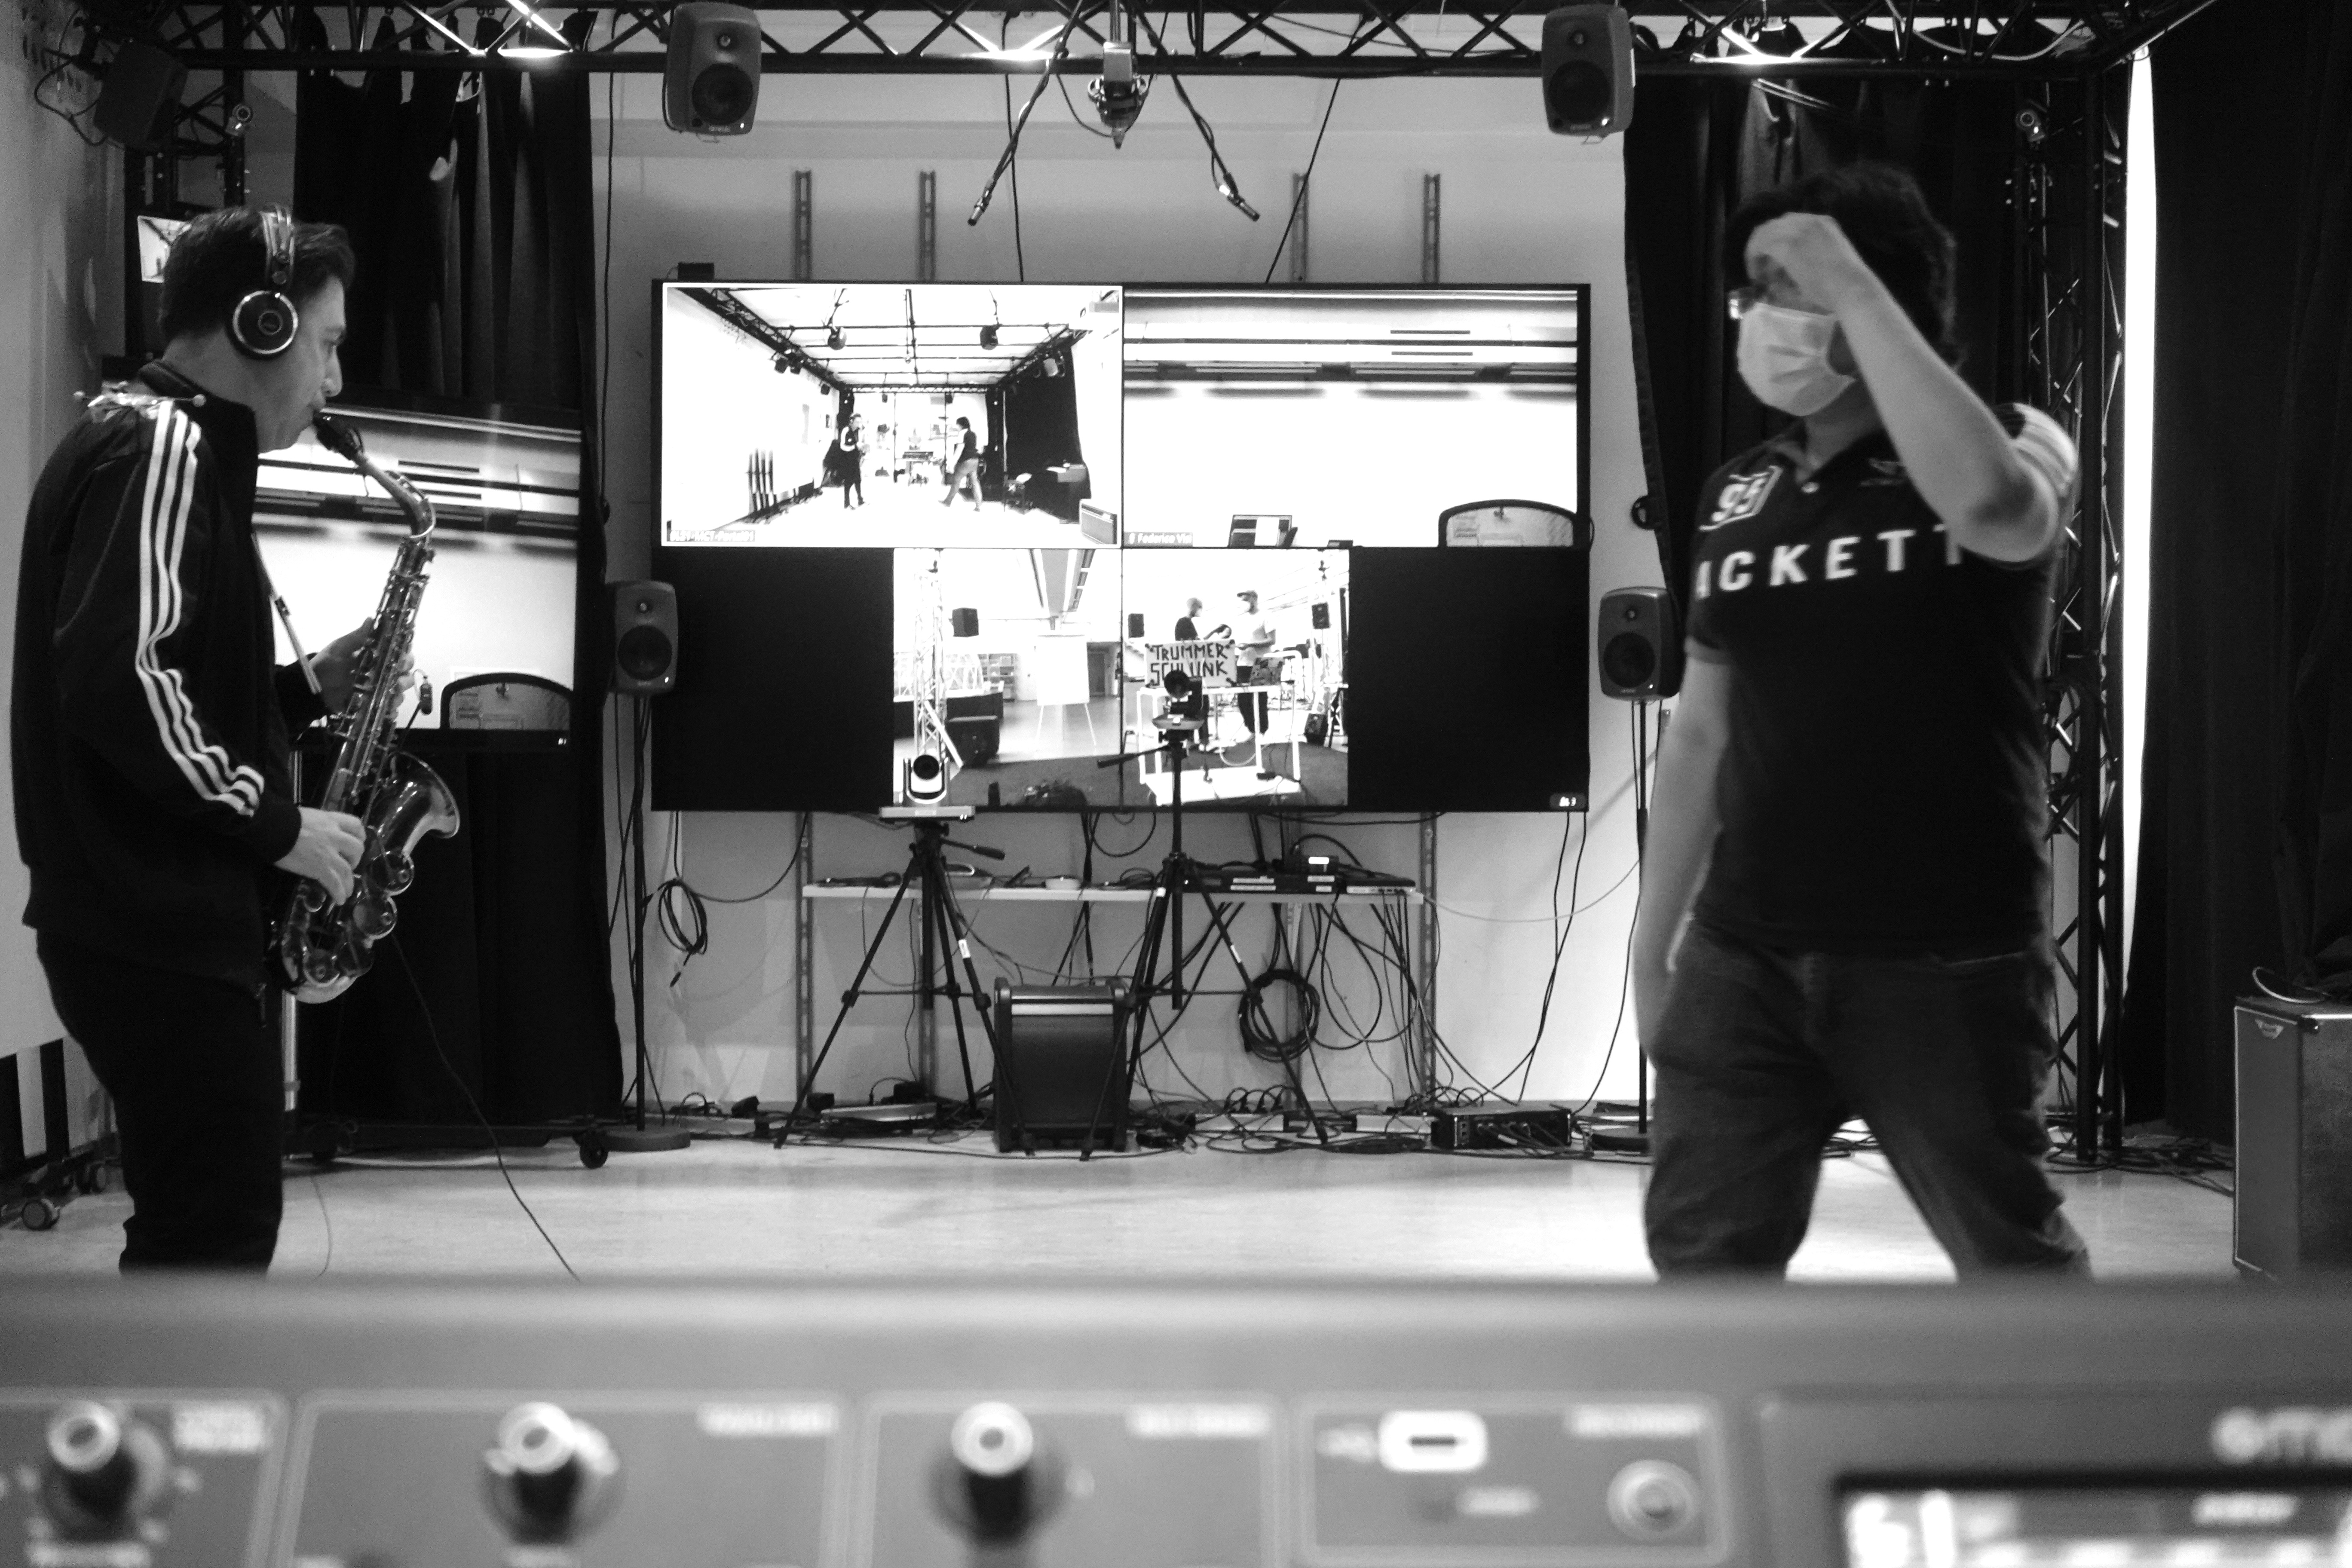
\includegraphics[width=\columnwidth]{figures/60-mct-portal.jpg}
	\caption{The MCT Portal, a laboratory for low-latency audiovisual communication at the University of Oslo. Here set up for a performance with musicians in Oslo, Berlin, and Stockholm in 2021.}
	\label{fig:portal}
\end{figure}

New technologies have allowed for increasing the distance between action and sound, both technologically and conceptually. Networking software such as Jacktrip \citep{caceres_jacktrip_2010} and LOLA \citep{drioli_networked_2013} have made it possible to explore high-quality and low-latency musicking. Now we also see the advent of digital mixers and commercial communication protocols such as Dante \citep{williams_network_nodate} and Network Device Interface (NDI) \citep{ellerbrock_network_nodate}. These standards make it possible to send audio and video over networks with a high level of synchronization between streams.
An interesting by-product of the development of network-based signaling is that it can also be used \emph{within} a concert space. The result is a setup that is both more complex and simple at the same time. More complex, digital technologies (for example, a digital stage box and mixer) can replace analog technologies (such as cabling and DI boxes). This will probably be seen as a simplification from the sound technician's point of view. It may be a transparent change of technologies for the musician on stage, unless the added latency is perceptually challenging. It would probably also lead to a better overall experience for the audience. The change to network-based technologise may also lead to new audience experiences, such as we have seen with the growth of online performances.

All in all, switching to digital technologies will, in many cases, lead to a better-sounding result and new musicking possibilities. However, there may be some added challenges related to an increased spatiotemporal distance. After all, musical co-performance relies on continuous \emph{inter}action with the fellow performers. A temporal lag in the others' sound and image makes it challenging to perform together. Anyone who has tried to perform using a conventional video conferencing system has experienced that latencies of a few hundred milliseconds make it challenging to play normal rhythms and melodies together. This is particularly the case if there is also an additional variation (jitter) of the latency. Delays in the signal may work for regular conversations but not for time-critical music performance. Thus it is essential to reduce the latency in all parts of the action--sound chain.

Paradoxically, sometimes the experienced latency may go down in telematic performance. For orchestra musicians spaced out on a large stage (30 meters wide), it takes approximately 90 milliseconds for the sound to travel from one side to the other. Suppose instead the sound from the instrument was captured with a microphone, digitized, sent through a network and played through headphones to another musician. In that case, they might have a smaller perceived latency than through analog transmission. This is not to say that symphony orchestras should switch to perform telematically, but it brings another perspective to the latency discussion.

Latency may be considered a drawback, but it may also be used creatively. The piece/instrument Superstring Theories by Øyvind Brandtsegg and Bernt Isak Wærstad
%todo: add reference?
can be considered a `telematic instrument' \citep{brandtsegg_towards_2022}. It is built around a physical string model that runs on two physically dislocated computers and uses the network latency between the two computers as a delay line in the sound engine. There are two human performers involved, one in each physical location, performing on a \emph{shared} instrument. This instrument can be seen as a development of the concept of \emph{cross-adaptive} performance \citep{brandtsegg_working_2018} in which the sound-producing actions performed on one instrument influence the timbre of another instrument. Such shared instruments are constructed around combinations of acoustic and electro-acoustic instruments. They use machine-based sound analysis methods to extract some sound features from one instrument applied to the other. Since the instrument is already based on a network---both conceptually and technically---they lend themselves well to telematic performance.

There are additional conceptual challenges when performing together in different locations. No rooms are the same, which means that the perceived ambiance of the spaces will differ. As \citep[p.424]{braasch_telematic_2009} reflects:

\begin{quotation}
[\ldots] our organism is formed by interacting with its environment. From a phenomenological viewpoint, it becomes much easier to treat the telematic system as a unique environment instead of a copy of another place, which a rationalist would call the ‘real’ or ‘physical’ world.
\end{quotation}

That is why we talk about the MCT Portal as a `physical-virtual' environment. The performers are co-located in two (or more) physical rooms connected with audiovisual technologies. Conceptually speaking, everyone is located in one common physical-virtual room. If you are on the physical Oslo side of the MCT Portal, you are at the same time virtually present in the other connected physical rooms and the other way around. While setting up the space, I was always concerned about creating a feeling of \emph{presence}, of being `together' with people on the other side of the communication chain. Too often, video conferencing setups lead to the experience of `us' and `them.' Rather, we should think about a common `we.' This is something that differentiates telematic performance from other types of performance. It is not only about `streaming' image and sound from one location to another. It is about creating a shared physical-virtual performance environment. You know that you are in your own physical environment, but you also know that you are elsewhere. Sometimes you know the other physical space well; other times, you are virtually present in physical locations that you do not know. Even with high-quality audiovisual representations of the other physical space, there is a difference between being physically and virtually present.

Telematic performance has been a niche activity for a long time but has nowadays become commonplace. Better technology helps, but also more knowledge about the positive sides of playing with people that are spatially dislocated from yourself. More than ten years ago \citep[p.2]{oliveros_telematic_2009} argued:

\begin{quotation}
As the technology improves exponentially and ubiquitously then eventually there will be no reason not to perform music at a distance. Globalization gives us more reason. Making music together makes friends.
\end{quotation}

%“With regard to haptic sensation, for example, we are restricted to close proximity in a physical environment, and consequently we cannot interact socially with many people at the same time through touch. In a virtual world, however, the proximity could be easily extended through haptic interfaces, providing a unique affordance for telematic music systems” (p.430-431 J. Braasch)

%“The relationship between “environment” and “actor” go beyond complementarity and scale, and might begin to include historical information about the actor or the instrument such as musical experience and subjective matters such as musical preference and taste. In this, culture enters into the possible affordances provided by the system.” (Tanaka et al., 2012, sec. Discussion, para 2)

As Oliveros notes, telematic performance is a way of connecting with other people. It could even be seen as an `inter-cultural instrument' according to \citet{alarcon_diaz_sensing_2019}. In the project INTIMAL, she explored telematics as an interface for `relational listening.' Here the idea was to explore how performing together, over long distances, could be a way of connecting with others. Her group of focus was Colombian immigrant women in Europe. They are both dislocated relative to their original home country (Colombia), but also currently dislocated in their various new home countries around Europe. Her project's final telematic performance was performed between the cities of Oslo, Barcelona, and London. % (Figure~\ref{fig:intimal}).
We spent a great deal of time testing out various communication types for the performance. There were performers and local audiences in each of the cities, so we could have created a `normal' multimedia-style telematic performance through transmitting and playing back sound and video in each location. However, we wanted to see whether it was possible to create separate and co-located experiences simultaneously. We ended up transmitting the voices of the performers, but these were only heard by the other performers. So all the performers heard each other, but each local audience only heard the voices of the performers in their physical room. The only common auditory element played back in the three sites were sonifications of the women's respiration. The performers wore wrist belts that captured their breathing. The data was sent as control messages to the other sites where it was sonified using abstract sound models and played back \citep{alarcon_diaz_ellos_2019}. As such, the result was three independent yet connected performances. They happened simultaneously but in different locations, and the content was a mix of the abstract, sonified breathing, and site-specific, context-dependent performance elements. This was a very different telematic performance. It was not only about streaming audiovisual information from one place to another. Instead, it considered the local environment and context, with the performers being the `mediator' of the content from the other side.

%\begin{figure}[tp]
%	\includegraphics[width=\columnwidth]{figures/09-spatiotemporality/intimal.png}
%	\caption{From the performance of INTIMAL in Oslo, London, and Barcelona \citep{alarcon_diaz_sensing_2019}.}
%	\label{fig:intimal}
%\end{figure}



%During the coronavirus crisis, telematic performance has moved from being a niche to a mainstream activity. Many of the technologies were already in place, but they had mainly been explored in experimental settings. Now they are repurposed to use in all sorts of ways.

%I find it interesting to witness the exploration of telematic performance concepts.

%Mobile phone apps may be the biggest driver of this development. One example here is the previously mentioned Ocarina app, which also has a telematic performance element. \citet{wang_artful_2018} describes how they developed Ocarina as a toy, binding people together. You can play yourself, but you can also see and hear what others are playing. Here the telematic element adds a feeling of community, just like an `orchestra' where multiple people play together.


\section{Space and time}

Telematic performances call for an expanded model of how one considers space and time in music. I here think about `space' as the experience of a physical \emph{place}. In acoustic musicking, the perceptual space often relates to the physical construction of the place. The room acoustics shape the overall musical experience for both performers and perceivers. Concert halls and churches are places that afford particular experiences of space. But any room or outdoor location will have unique sonic characteristics. As discussed in Chapter~\ref{sec:space}, some environments can even be thought of as having instrument-like qualities, such as the entrance of Nationaltheatret train station in Oslo (Figure~\ref{fig:nationaltheatret}).

The question about space and place is more complicated in the world of electro-acoustic musicking. It is common to build `dry' rooms and add artificial environmental sound through the use of reverb and other sound effects. Some electro-acoustic instruments also have built-in reverb units to add spatiality to the output sound. Together this creates a mix of different spatial layers of sound:

\begin{enumerate}
	\item Physical resonance in the instrument
	\item Artificial reverb in the instrument
	\item Physical resonance in the room
	\item Artificial room reverb
\end{enumerate}

In the case of telematic performance, all (or some) of these layers may be transmitted to the other side. They will be mixed and played over speakers in a different physical room with its acoustic characteristics. Analyzing the complete sound chain and how it is perceived is a complicated task. I find it helpful to think about what \citet{moore_sonic_2016} calls the `space in sound' and `space through sound.' His approach, however, is coming from the perspective of composing. I am more interested in how we can think about space and place in a performance context. %This is very much based on the sonic qualities of music, however, as is \citet{holbrook_sound_2019} argumentation for a particular extension of Schaeffer's thinking about the sound object.
%These theories often tend to think about \emph{pieces} of music.

Traditional musical instruments, from guitar to synthesizer, are objects that are physically co-located with the performer. In most cases, the spatial dislocation is minimal in acoustic instruments, and the time delay is short. Electro-acoustic instruments may have a larger spatial dislocation between action and sound. They may also have different time delays. As described above, a musician on stage may have a stage monitor close to the instrument or an in-ear headset. This reduces the time delay of the action--sound (or sound--sound) mapping for the musician. However, the audience may experience both spatial dislocation and time delay if the speakers in the PA system are far from the performer.

The spatiotemporal distances found in telematic performance are of an entirely different magnitude. Here questions about in-time and out-of-time performance are more prevalent. However, the difference between the physical dislocation may not be proportional to the experienced latency. In the MCT Portal, we have optimized both the audiovisual setup and the network. This makes it possible to have a latency down to around 20 milliseconds between the cities of Oslo and Trondheim (500 kilometers apart). Speaking into a microphone in Oslo will result in sound output from a speaker in Trondheim with less experienced latency than if you sit in the back of a large concert hall. A latency of around 20 milliseconds is also fine for performing most types of musics together.

\section{`Here' and `now'}

When is the `now' when performing telematically? The performance is happening in real-time on both sides, but whose in-time would be the reference? Can we talk about a common `now'? This may be thought of as similar to the question of when lightning happens. There are multiple `nows' that refer to each other. When I perform in the MCT Portal, I have my experience of performing in-time. I am also aware that the performer on the other side has a different in-time experience than myself. It is common that both performers feel `dragged' towards the other's in-time. So when performing telematically it is necessary to resist slowing down to follow each other's in-time experience.

%\citet{barbosa_displaced_2003} separates between \emph{remote} and \emph{co-located} space in telematic performance.
In the MCT Portal, we try to create the experience of a physical-virtual `here,' even though everyone involved knows that there are multiple `here' and `there.' In my experience, it helps to keep the communication channels running continuously. Video conferencing systems are often based on the idea of `calling' someone else or `connecting' to a different room. This underlines the idea of a `here' and `there.' Instead, by leaving two (or more) locations connected continuously, you create a sense of togetherness. If you know that audio and video is transmitted, you enter a room with a different attitude. You know that when stepping into the room you are part of a physical-virtual `here.'

To connect my thinking about space to that of time, I will suggest two new terms: \emph{in-space} and \emph{out-of-space}. As for the terms in-time and out-of-time, these spaceterms also require `here' as a reference point. When performing telematically, my `here' and `now' is different from my co-performers' `here' and `now.' At the same time, we will both have an understanding of the other being `out-of-space' and `out-of-time' with respect to ourselves. We can play together because we are aware of each other's reference points.

However, being aware may not be sufficient in all cases. If the spatiotemporal distance gets to large, it may be impossible to play together in-time. Then it may be necessary to resolve to other types of performance modes in which timing is less important. The user may still feel connected to the others. \citet{swarbrick_how_2019} investigated people's experiences with live versus recorded music. They found that people enjoyed live music more, possibly because they increased anticipation and feelings of involvement for the audience.

%The question of time is, of course, also related to the question of \emph{space}.The model in Figure~\ref{fig:barbosa}, adapted from \citet{barbosa_displaced_2003}, is interesting in this respect. As can be seen in  he separates between \emph{synchronous} and \emph{asynchronous} time, and \emph{remote} and \emph{co-located} space.

%\begin{figure}[tp]
%	\includegraphics[width=\columnwidth]{figures/09-spatiotemporality/barbosa-crop.pdf}
%	\caption{An overview of different types of musicking within a space--time display. Adapted from a model presented in \citep{barbosa_displaced_2003}.}
%	\label{fig:barbosa}
%\end{figure}

%\subsection{The sound of the environment}

%There are also many examples of how space has been developed into a musical parameter. Much of the experimentation in `tape music' has been focused on creating virtual spaces. They have been diffused on different types of speaker orchestras. The size, quality, and placement of the speakers is a core part of the musical output. The instrument in such a context would be a combination of all the speakers. Since so much of the musical output focuses on the location, distribution, and timbral qualities of the space within which it is performed, the space itself would play an essential part of the sound.




%When it comes to It is the boundary between acoustic and electro-acoustic instruments that I find most exciting to explore further. Many acoustic instruments are amplified in performance these days. According to my definition, we should then consider them as electro-acoustic instruments and include the microphone and speaker system in our analysis of the whole action--sound chain. This expands our understanding of the spatiotemporal nature of the performance. New technologies allow for an increased spatial and temporal dislocation of action and sound. In the most extreme cases---such as telematic performance---one can perform with a controller in one country and a sound engine in another. However, are there any limitations on the spatial distance or temporal lag of an instrument? If I press a key in Norway today that results in a sound being played in Chile tomorrow, is that an instrument? In theory, only the spatiotemporal scale differentiates it from pressing a key that results in sound today `here' and `now.' This and similar questions arise more frequently as telematic performance is gaining traction. I will leave these questions unanswered here and call for others to continue the theoretical development.
